%Copyright 2019 Christopher M. Jermaine (cmj4@rice.edu) and Risa B. Myers (rbm2@rice.edu)
%
%Licensed under the Apache License, Version 2.0 (the "License");
%you may not use this file except in compliance with the License.
%You may obtain a copy of the License at
%
%    https://www.apache.org/licenses/LICENSE-2.0
%
%Unless required by applicable law or agreed to in writing, software
%distributed under the License is distributed on an "AS IS" BASIS,
%WITHOUT WARRANTIES OR CONDITIONS OF ANY KIND, either express or implied.
%See the License for the specific language governing permissions and
%limitations under the License.

\documentclass[aspectratio=169]{beamer}

%===============================================================%
\mode<presentation> 
{
\usetheme[noshadow, minimal,numbers,riceb,nonav]{Rice}
\usefonttheme[onlymath]{serif}
\setbeamercovered{transparent}
}
\useinnertheme{rectangles}

\usepackage[english]{babel}

\usepackage{mathptmx}
\usepackage{helvet}
\usepackage{courier}
\usepackage[T1]{fontenc}
\usepackage{trajan}
\usepackage{textcomp}

\usepackage{listings}

\newenvironment{noindentitemize}
{ \begin{itemize}
 \setlength{\itemsep}{1.5ex}
  \setlength{\parsep}{0pt}   
  \setlength{\parskip}{0pt}
 \addtolength{\leftskip}{-2em}
 }
{ \end{itemize} }

\newenvironment{noindentitemize2}
{ \begin{itemize}
  \setlength{\itemsep}{0ex}
  \setlength{\parskip}{0pt}
  \setlength{\parsep}{0pt}   
  \addtolength{\leftskip}{-2em}  }
{ \end{itemize} }



\setbeamerfont{block body}{size=\tiny}

%===============================================================%

\title[]
{Tools \& Models for Data Science}

\subtitle{Introduction to Relational Databases}

\author[]{Chris Jermaine \& Risa Myers}
\institute
{
  Rice University
}

\date[]{}

\subject{Beamer}


\begin{document}

\begin{frame}
 \titlepage
\end{frame}


\begin{frame}{What is a Database?}

\begin{itemize}
\item A collection of data
\item Plus, a set of programs for managing that data
\end{itemize}
\end{frame}
%***********************************************************

\begin{frame}{Back in the Day...}

\begin{itemize}
\item The dominant data model was the network or navigational model (60's and 70's)
\item Data were a set of records with pointers between them
\item Much DB code was written in COBOL
\item Big problem was lack of physical data independence
	\begin{itemize}
	\item Code was written for specific storage model
	\item Want to change storage?  Modify your code
	\item Want to index your data?  Modify your code
	\item Led to very little flexibility
		\begin{itemize}
		\item Your code locked you into a physical database design!
		\end{itemize}
	\end{itemize}
\end{itemize}
\end{frame}

%***********************************************************
\begin{frame}{Some People Realized This Was a Problem}

\begin{itemize}
\item By 1970, EF Codd (IBM) was looking at the so-called relational model
	\begin{itemize}
	\item Landmark 1970 paper, ``A relational model of data for large shared data banks''
	\item Led to the 1981 Turing Award
		\begin{itemize}
		\item Highest honor a computer scientist receives
		\item Analogous to a Nobel Prize
		\end{itemize}
	\end{itemize}
\item Idea: data stored in ``relations'' 
	\begin{itemize}
	\item A relation is a table of tuples or records
	\item Attributes of a tuple have no sub-structure (are atomic)
	\end{itemize}
\item No pointers!
\end{itemize}
\end{frame}

%***********************************************************
\begin{frame}{Databases are Still Important}

\begin{itemize}
\item 2014, Michael Stonebraker
	\begin{itemize}
	\item ``For fundamental contributions to the concepts and practices underlying modern database systems" 
	\item Led to the 2014 Turing Award
		\begin{itemize}
		\item INGRES relational database system in 1974, based on Codd's papers
		\item Inspired numerous other database systems, including Postgres
		\end{itemize}
	\end{itemize}
\end{itemize}
\end{frame}
%***********************************************************
\begin{frame}{Key RDBMS Features}

\begin{itemize}
\item Querying
\item ACID properties
	\begin{itemize}
	\item Atomicity
	\item Consistency
	\item Isolation
	\item Durability
	\end{itemize}
\end{itemize}
\end{frame}
%***********************************************************
\begin{frame}{Querying in the Relational Model}

\begin{itemize}
\item Querying is done via a ``relational calculus''
\item Declarative
	\begin{itemize}
	\item You give a mathematical description of the tuples you want
	\item System figures out how to get those for you
	\end{itemize}
\item[?] Why is this good?
\end{itemize}
\end{frame}

%***********************************************************
\begin{frame}{Querying in the Relational Model}

\begin{itemize}
\item Querying is done via a ``relational calculus''
\item Declarative
	\begin{itemize}
	\item You give a mathematical description of the tuples you want
	\item System figures out how to get those for you
	\end{itemize}
\item[?] Why is this good?
	\begin{itemize}
	\item Data independence!
	\item Your code has no data access specifications
	\item You can change the physical organization with no code re-writes	
	\end{itemize}
\end{itemize}
\end{frame}

%***********************************************************
\begin{frame}{Relational Schema}

\begin{itemize}
\item All data are stored in tables, or relations
\item A relation schema consists of:
	\begin{itemize}
	\item A relation name (e.g., LIKES)
	\item A set of (attribute\_name, attribute\_type) pairs
		\begin{itemize}
		\item Each pair is referred to as an ``attribute''
		\item Or sometimes as a ``column''
		\end{itemize}
	\item Usually denoted using \\
	LIKES (DRINKER string, COFFEE string)
	\item Or simply LIKES (DRINKER, COFFEE)
	\end{itemize}
\end{itemize}
\end{frame}

%***********************************************************
\begin{frame}{A Relation}

\begin{itemize}
\item A relation schema defines a set of sets
	\begin{itemize}
	\item Specifically, if $T_1, T_2, ..., T_n$ are the $n$ attribute types
	\item Where each $T_i$ is a set of possible values
		\begin{itemize}
		\item Ex: string is all finite-length character strings
		\item Ex: integer is all numbers from $-2^{31}$ to $2^{31} - 1$
		\end{itemize}
	\item Then a realization of the schema (aka a ``relation'') is a subset of
		\begin{itemize}
		\item $T_1 \times T_2 \times ... \times T_n$
		\item where $\times$ is the Cartesian product operator
		\end{itemize}
	\end{itemize}
\end{itemize}
\end{frame}
%***********************************************************
\begin{frame}{Attribute Types Forming a Relation}

{\centering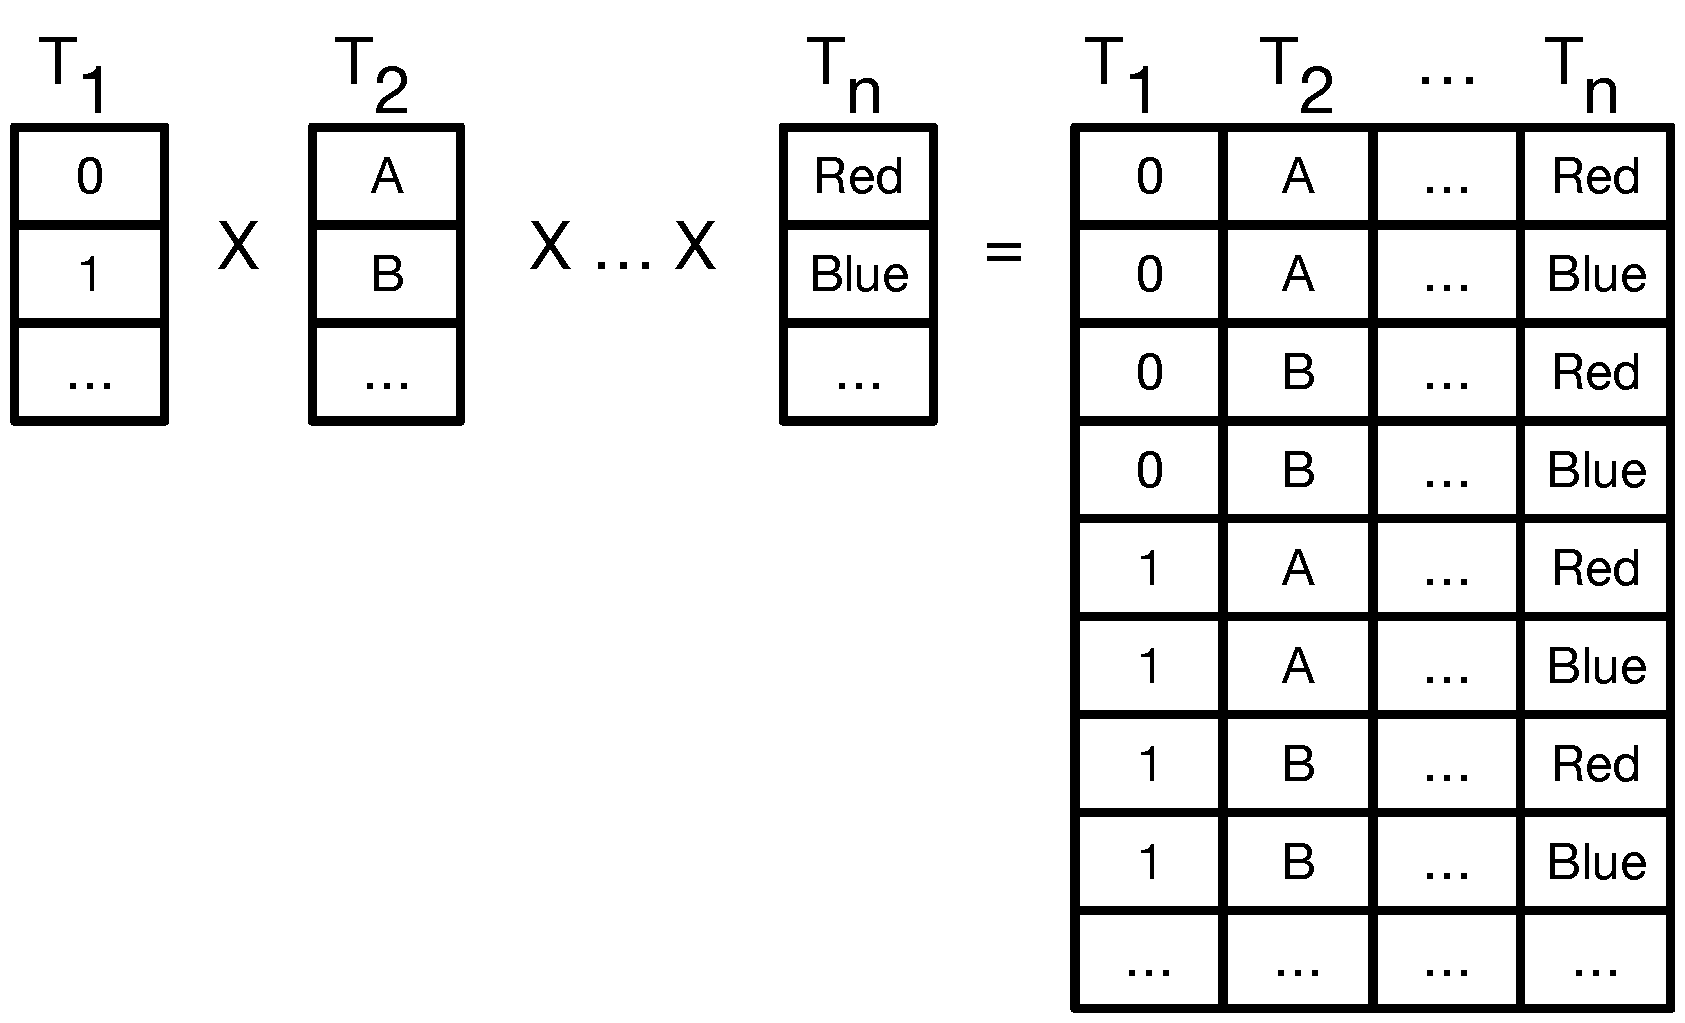
\includegraphics[width=0.8\textwidth]{./lectRDBMS/attributeTypes.pdf}\par}


However, not all tuple combinations actually occur
\end{frame}

%***********************************************************
\begin{frame}{A Relation (continued)}

\begin{itemize}
\item So for the relation schema\\ LIKES (DRINKER string, COFFEE string)
\item A corresponding relation might be
	$$\{(\textrm{\textquotesingle{Chris}\textquotesingle, \textquotesingle{Espresso\textquotesingle}}), \textrm{(\textquotesingle{Risa}\textquotesingle, \textquotesingle{Cold Brew}\textquotesingle)}\}$$
\item This is also referred to as a ``table''
\item The entries in the relation are referred to as
	\begin{itemize}
	\item ``rows''
	\item ``tuples'' % mathematical
	\item ``records'' % physical
	\end{itemize}
\end{itemize}
\end{frame}
%***********************************************************
\begin{frame}{Relational Terminology}

{\centering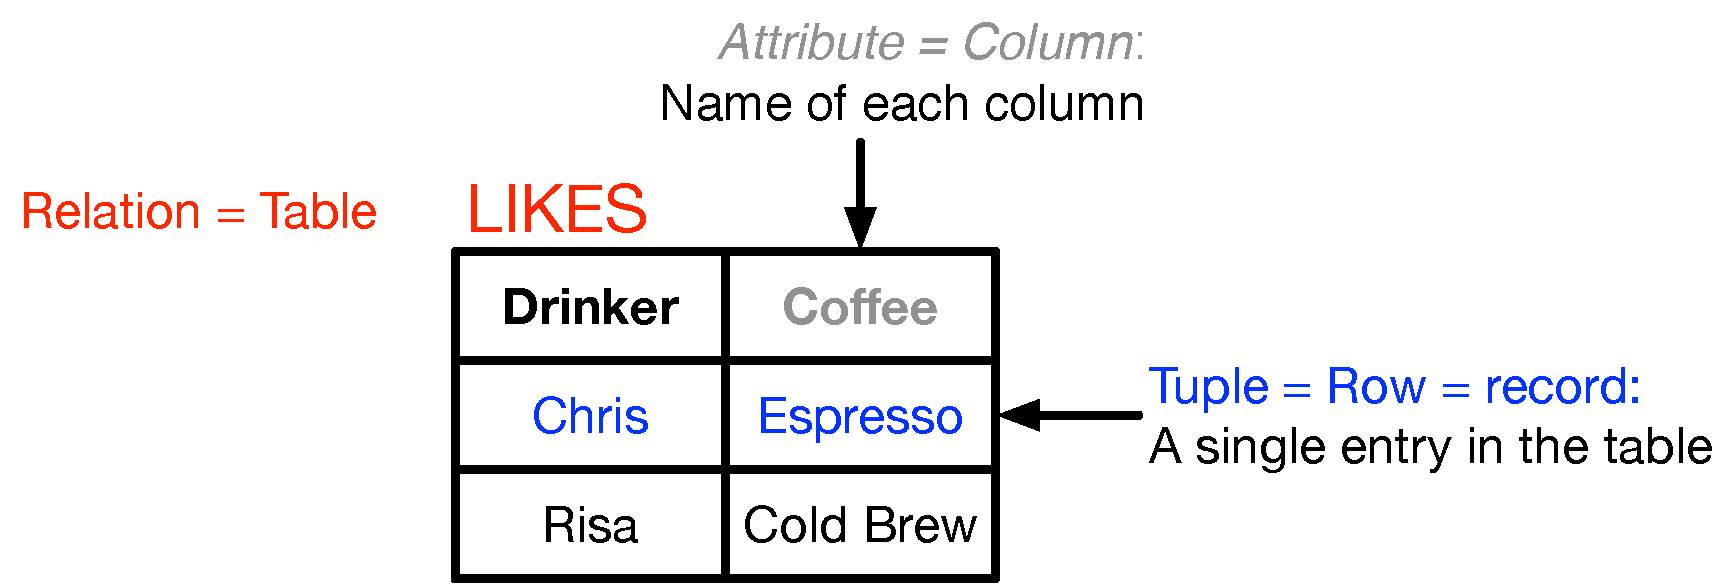
\includegraphics[width=1\textwidth]{./lectRDBMS/terminology.pdf}\par}
\end{frame}

%***********************************************************
\begin{frame}{Keys}

\begin{itemize}
\item In the relational model, given $R(A_1, A_2, ..., A_n)$
\item A set of attributes $K = \{K_1, ..., K_m\}$ is a KEY of $R$ if:
	\begin{itemize}
	\item For any valid realization $R'$ of $R$...
	\item For all $t_1, t_2$ in $R'$...
	\item If $t_1[K_1] = t_2[K_1]$ and $t_1[K_2] = t_2[K_2]$ and ... 
		$t_1[K_m] = t_2[K_m]$...
	\item Then it must be the case that $t_1 = t_2$ 
	\end{itemize}
\item[?] Note: every relation schema SHOULD have a key... why?
\end{itemize}
\end{frame}
%***********************************************************
\begin{frame}{Keys: Exercise}
\begin{itemize}
\item[?] What is a key for \\STUDENT (NETID, FNAME, LNAME, AGE, COLLEGE)?

\end{itemize}
\end{frame}
%***********************************************************
\begin{frame}{Keys: Exercise}
\begin{itemize}
\item[?] What is a key for \\ LIKES (DRINKER, COFFEE)?
\end{itemize}
\end{frame}
%***********************************************************
\begin{frame}{Keys: Exercise}
\begin{itemize}
\item What is a key for \\ LIKES (DRINKER, COFFEE)?

What is the relation about?\\
Is it about a drinker's favorite style of coffee?\\
Or about the first person to drink a coffee?\\
Or about what styles of coffee does each drinker like?\\
Context matters!\\
% In this course, you will be give the data in relations already, but somet
\end{itemize}
\end{frame}


%***********************************************************
\begin{frame}{Keys (continued)}

\begin{itemize}
\item A relation schema can have many keys
\item Those that are minimal are \textbf{CANDIDATE KEY}s
	\begin{itemize}
	\item ``Minimal'' means no subset is a key
	\end{itemize}
\item One is typically designated as the \textbf{PRIMARY KEY} 
\item This key typically determines the order in which the data are stored 
\item Denoted with an underline
	\begin{itemize}
	\item STUDENT (\underline{NETID}, FNAME, LNAME, AGE, COLLEGE)
	\end{itemize}
\end{itemize}
\end{frame}

%***********************************************************
\begin{frame}{Connecting Relations}

The relational model does not have pointers that connect different relations\\
\vspace{1em}
\begin{itemize}
\item[?] Why not? 
\end{itemize}

\end{frame}

%***********************************************************
\begin{frame}{Connecting Relations}

The relational model does not have pointers that connect different relations\\
\vspace{1em}
Why not? 
	\begin{enumerate}
	\item Not nice mathematically 
		\begin{itemize}
		\item Mathematical elegance key goal in model design
		\end{itemize}
	\item Difficult implementation 
		\begin{itemize}
		\item Move an object?  All pointers are invalid!
		\item Solution: Use  a centralized look-up table
		\begin{itemize}
		\item Expensive
		\item Complicated
		\item Problem still exists	
		\end{itemize}
		\end{itemize}
	\end{enumerate}
\end{frame}

%***********************************************************
\begin{frame}{Solution: Foreign Keys}

\begin{itemize}
\item But we still need some notion of between-tuple references
	\begin{itemize}
	\item LIKES (DRINKER, COFFEE)
	\item DRINKER (DRINKER, FNAME, LNAME)
	\item Clearly, LIKES.DRINKER refers to DRINKER.DRINKER
	\end{itemize}
\item Accomplished via the idea of a FOREIGN KEY
\end{itemize}
\end{frame}

%***********************************************************
\begin{frame}{Foreign Keys (continued)}

\begin{itemize}
\item Given a relation schema: $R_1$, $R_2$
	\begin{itemize}
	\item We say a set of attributes $K_1$ from $R_1$ is a foreign key to a set of 
		attributes $K_2$ from $R_2$ if...
	\item (1) $K_2$ is a candidate key for $R_2$, and...
	\item (2) For any valid realizations $R_1'$, $R_2'$ of $R_1$, $R_2$...
	\item For each tuple $t_1 \in R_1'$, it MUST be the case that there exists $t_2 \in R_2'$ s.t...
	\item $t_1[K_{1,1}] = t_2[K_{2,1}]$ and $t_1[K_{1,2}] = t_2[K_{2,2}]$ and ...
                $t_1[K_{1,m}] = t_2[K_{2,m}]$
	\end{itemize}
\item[?] Intuitively, what does this mean?


{\centering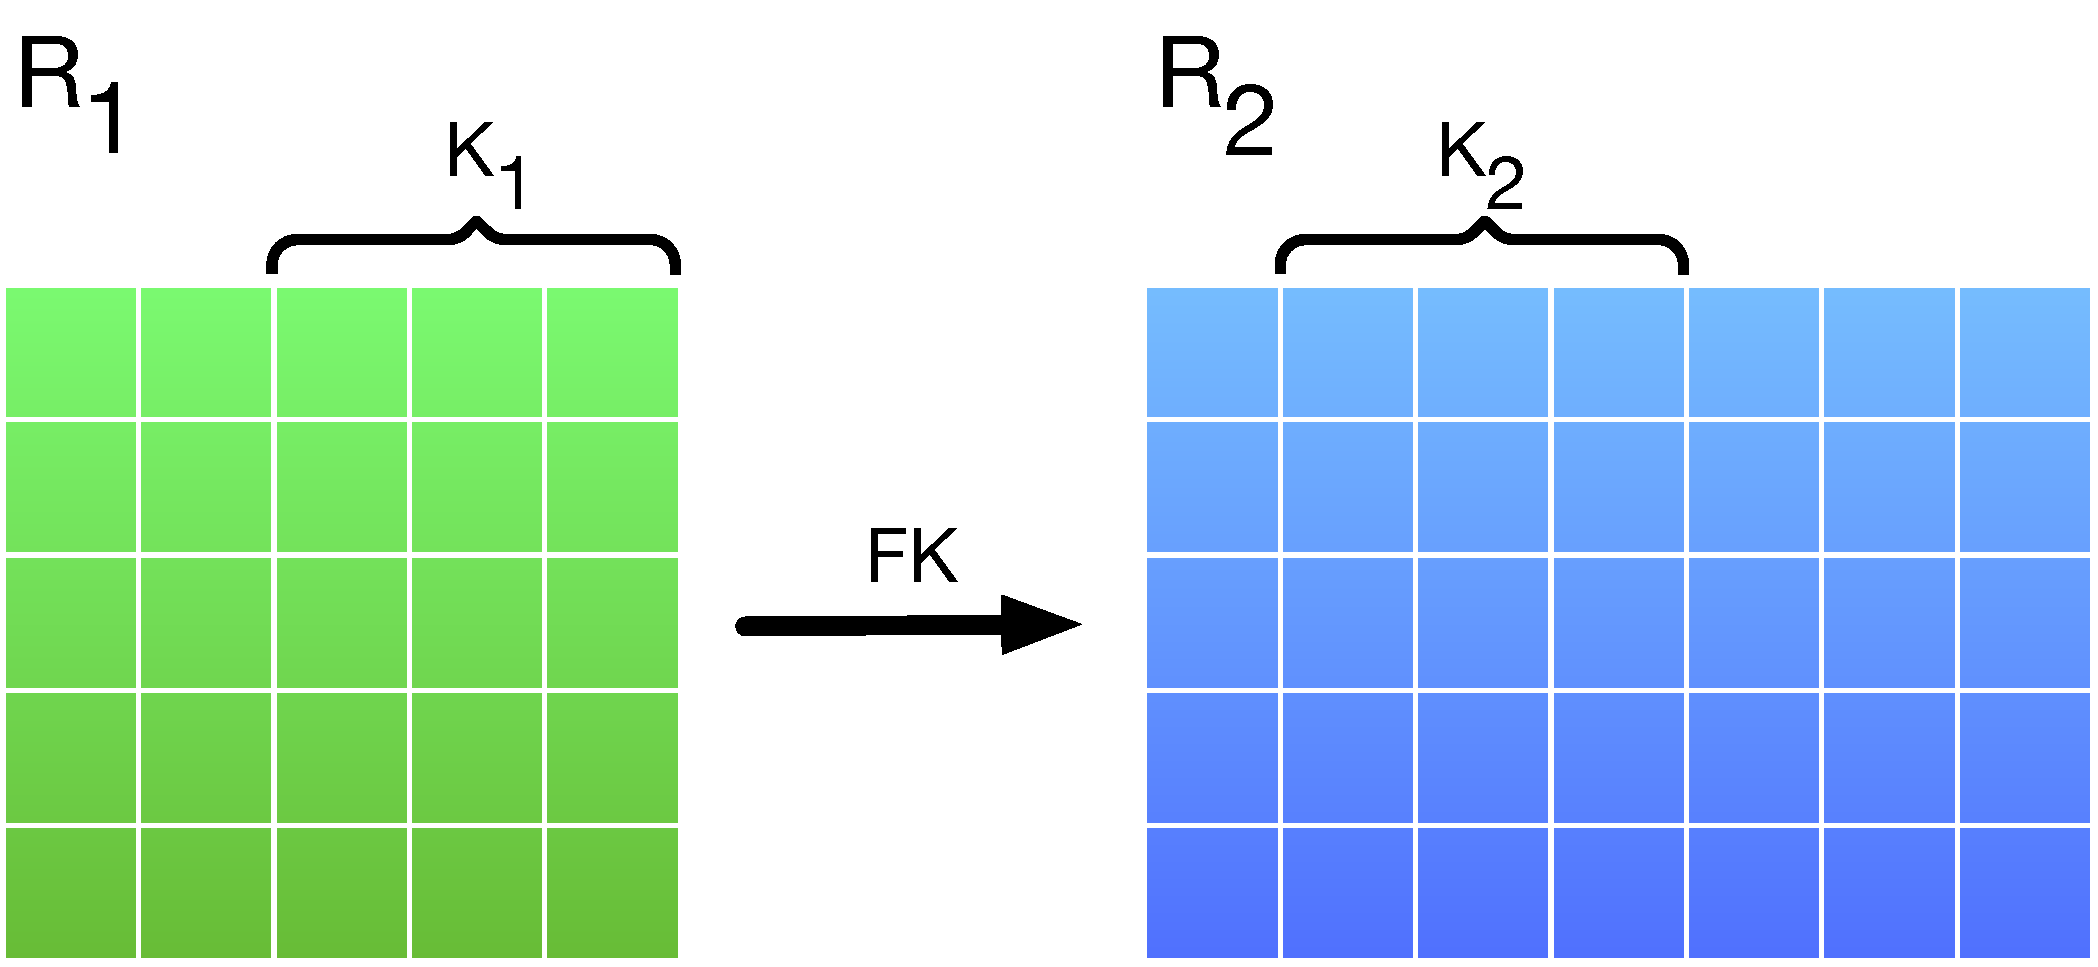
\includegraphics[width=.5\textwidth]{./lectRDBMS/fk.pdf}\par}

\end{itemize}
\end{frame}
%***********************************************************
\begin{frame}{Foreign Key Interpretation}

Intuitively, what does this mean?
\begin{itemize}
\item The foreign key must be an attribute or set of attributes that uniquely identify a record in another table
\item AND that combination of attribute values must be present in the other table
\item The foreign key may consist of
	\begin{itemize}
	\item More than one attribute
	\item Attributes with different names in each table
	\end{itemize}
\vspace{2em}
\item[?] Which way is the foreign key?
% LIKES has a FOREIGN KEY to PERSON
% It can't go the other direction, since netId is not a unique key in LIKES
\end{itemize}
\vspace{2em}
{\scriptsize
\begin{columns}
\begin{column}{0.5\textwidth}
PERSON\\
\begin{tabular}{|l|l|l|l| }  \hline
\textrm{NETID} & \textrm{FIRSTNAME}& \textrm{LASTNAME}\\ \hline
{\color{red}cmj4} & Chris & Jermaine  \\ \hline
{\color{blue}rbm2} & Risa & Myers\\ \hline
\end{tabular}\\

\end{column}
\begin{column}{0.5\textwidth}
LIKES\\
\begin{tabular}{|l|l|}  \hline
\textrm{DRINKER} & \textrm{COFFEE}\\ \hline
{\color{red}cmj4} & Espresso  \\ \hline
{\color{blue}rbm2}  & Cold Brew \\ \hline
{\color{red}cmj4} & Chai Latte  \\ \hline
\end{tabular}\\
\end{column}
\end{columns}
}
\end{frame}

%***********************************************************
\begin{frame}{Foreign Key Interpretation}
\begin{itemize}
\item In other words
\begin{itemize}
\item The target must be a candidate key
\item There are no dangling pointers
\end{itemize}
\item[?] Why is this a requirement?
\end{itemize}

\end{frame}
%***********************************************************
\begin{frame}{Foreign Key Interpretation}
\begin{itemize}
\item In other words
\begin{itemize}
\item The target must be a candidate key
\item There are no dangling pointers
\end{itemize}
\item Why is this a requirement?
\begin{itemize}
\item To prevent inconsistencies
\item To match to a single target
\end{itemize}
\item The database enforces these requirements via
\begin{itemize}
\item Cascading deletes
\item Failed inserts
\end{itemize}
\end{itemize}

\end{frame}

%***********************************************************
\begin{frame}{Queries/Computations in the Relational Model}

\begin{noindentitemize}
\item The original query language was the RELATIONAL CALCULUS
	\begin{noindentitemize2}
	\item Fully declarative programming language
	\item Mostly theoretical/math  -- not actually implemented
	\item Helps you understand how to write SQL
	\end{noindentitemize2}
\item next was the RELATIONAL ALGEBRA
	\begin{noindentitemize2}
	\item Imperative
	\item Define a set of operations over relations
	\item An RA program is then a sequence of those operations
	\item This is the ``abstract machine'' of RDBs
	\item Helps you understand query performance
	\end{noindentitemize2}
\end{noindentitemize}
\end{frame}
%***********************************************************
\begin{frame}{Queries/Computations in the Relational Model}
\begin{noindentitemize}
\item Today we use SQL
	\begin{noindentitemize2}
	\item Heavily influenced by RC
	\item Has aspects of RA
	\item More complex than either of them!
	\end{noindentitemize2}
\end{noindentitemize}

\end{frame}

%***********************************************************
\begin{frame}{Overview of Relational Calculus}

\begin{itemize}
\item RC is a variant on first order logic
\item You say: ``Give me all tuples $t$ where $P(t)$ holds''
\item $P(t)$ is a predicate in first order logic
\end{itemize}
\end{frame}

%***********************************************************
\begin{frame}{Predicates}

\begin{itemize}
\item First order logic allows predicates
	\begin{itemize}
	\item Predicate: A function that evals to true/false
	\item ``It's raining on day X'' or $Raining(X)$
	\item ``It's cloudy on day X'' or $Cloudy(X)$
	\end{itemize}
\item Build more complicated predicates using logical operations over them
	\begin{itemize}
	\item and ($\wedge$) (both)
	\item or ($\vee$)	(either or both)
	\item not ($\neg$)	(flip truth value)
	\item implies ($\rightarrow$)
	\item if and only if ($\leftrightarrow$)
	\end{itemize}
\end{itemize}
\end{frame}

%***********************************************************
\begin{frame}{Predicates: And}
\begin{columns}[t]
\begin{column}{0.6\textwidth}
$Raining(X) \wedge Cloudy(X)$
Evaluates to TRUE if both:
\begin{itemize}
\item It is raining on day X\\
and
\item It is cloudy on day X
\end{itemize}
\end{column}
\begin{column}{0.4\textwidth}
AND Truth Table\\
\begin{tabular}{|l|c||c| }  \hline
\textbf{p} & \textbf{q} & \textbf{p $\wedge$ q}\\ \hline
T & T & T\\ \hline
T & F & F\\ \hline
F & T & F\\ \hline
F & F & F\\ \hline
\end{tabular}
\end{column}
\end{columns}
\end{frame}

%***********************************************************
\begin{frame}{Predicates: Or}
\begin{columns}[t]
\begin{column}{0.6\textwidth}
$Raining(X) \wedge Cloudy(X)$
Evaluates to TRUE if either:
\begin{itemize}
\item It is raining on day X\\
or
\item It is cloudy on day X
\end{itemize}
\end{column}
\begin{column}{0.4\textwidth}
OR Truth Table\\
\begin{tabular}{|l|c||c| }  \hline
\textbf{p} & \textbf{q} & \textbf{p $\vee$ q}\\ \hline
T & T & T\\ \hline
T & F & T\\ \hline
F & T & T\\ \hline
F & F & F\\ \hline
\end{tabular}
\end{column}
\end{columns}
\end{frame}

%***********************************************************
\begin{frame}{Predicates: Implies}
\begin{columns}[t]
\begin{column}{0.6\textwidth}
$Raining(X) \rightarrow Cloudy(X)$\\
Evaluates to TRUE if either:
\begin{itemize}
\item It is not raining on day X\\
or
\item It is raining and cloudy on day X
\item $\rightarrow$ is like a logical ``if-then''
\item State is FALSE if it is raining and not cloudy
\item If it's not raining, we don't care about whether or not it's cloudy
\end{itemize}
\end{column}
\begin{column}{0.4\textwidth}
IMPLICATION\\Truth Table\\
\begin{tabular}{|l|c||c| }  \hline
\textbf{p} & \textbf{q} & \textbf{p $\rightarrow$ q}\\ \hline
T & T & T\\ \hline
T & F & F\\ \hline
F & T & T\\ \hline
F & F & T\\ \hline
\end{tabular}
\end{column}
\end{columns}
\end{frame}

%***********************************************************
\begin{frame}{Predicates: If and Only If}

Raining(X) $\leftrightarrow$ Cloudy(X)
Evaluates to TRUE if both:
\begin{itemize}
\item Raining(X) $\rightarrow$ Cloudy(X)\\
AND
\item Cloudy(X) $\rightarrow$ Raining(X)\\
\end{itemize}

\vspace{2em}
IFF Truth Table\\
\begin{tabular}{|c|c|c|c||c|}  \hline
\textbf{p} & \textbf{q} & \textbf{p $\rightarrow$ q} & \textbf{q $\rightarrow$ p} & \textbf{p $\leftrightarrow$ q}\\ \hline
T & T & T &  T & T\\ \hline
T & F & F & T & F\\ \hline
F & T & T & F & F\\ \hline
F & F & T & T & T \\ \hline
\end{tabular}
\end{frame}





%%***********************************************************
%\begin{frame}{Predicates (continued)}
%
%\begin{itemize}
%\item Example: $Raining(X) \rightarrow Cloudy(X)$
%\item Evaluates to true if either:
%	\begin{itemize}
%	\item It is not raining on day $X$, or
%	\item It is raining and cloudy on day $X$
%	\end{itemize}
%\item Example: $Raining(X) \wedge Cloudy(X)$
%\item Evaluates to true if:
%	\begin{itemize}
%	\item It is raining and cloudy on day $X$
%	\end{itemize}
%\item Note the difference between them!
%	\begin{itemize}
%	\item $\rightarrow$ is like a logical ``if-then''
%	\end{itemize}
%\end{itemize}
%\end{frame}

%***********************************************************
\begin{frame}{First Order Logic}

\begin{itemize}
\item Just predicates and logical ops?
	\begin{itemize}
	\item You've got predicate logic
	\end{itemize}
\item But when you add quantification
	\begin{itemize}
	\item $\forall$, $\exists$
	\item You've got first order logic 
	\end{itemize}
\end{itemize}
\end{frame}

%***********************************************************
\begin{frame}{Universal Quantification}

\begin{itemize}
\item Asserts that a predicate is true all of the time
\item Example:
	\begin{itemize}
	\item $\forall(X)(Raining(X) \rightarrow Cloudy(X))$
	\item Zero-argument predicate (takes no params)
	% Yes, Zero Args, because X is assigned to each item in the UofD iteratively
	\item Asserts that it only rains when it is cloudy
	\item Note: idea of universe of discourse is key!
	\item X is a variable. It ranges over the entire universe of discourse
	\item Plug the value of that variable into the predicate. If it is always true, then the predicate is true

	\end{itemize}
\end{itemize}
\end{frame}

%***********************************************************
\begin{frame}{Universal Quantification Example 1}

\begin{itemize}
\item $\forall(X)(Raining(X) \rightarrow Cloudy(X))$
\item Given the following Universe of Discourse, is our predicate T or F?
\end{itemize}
\begin{columns}
\begin{column}{0.5\textwidth}
{\centering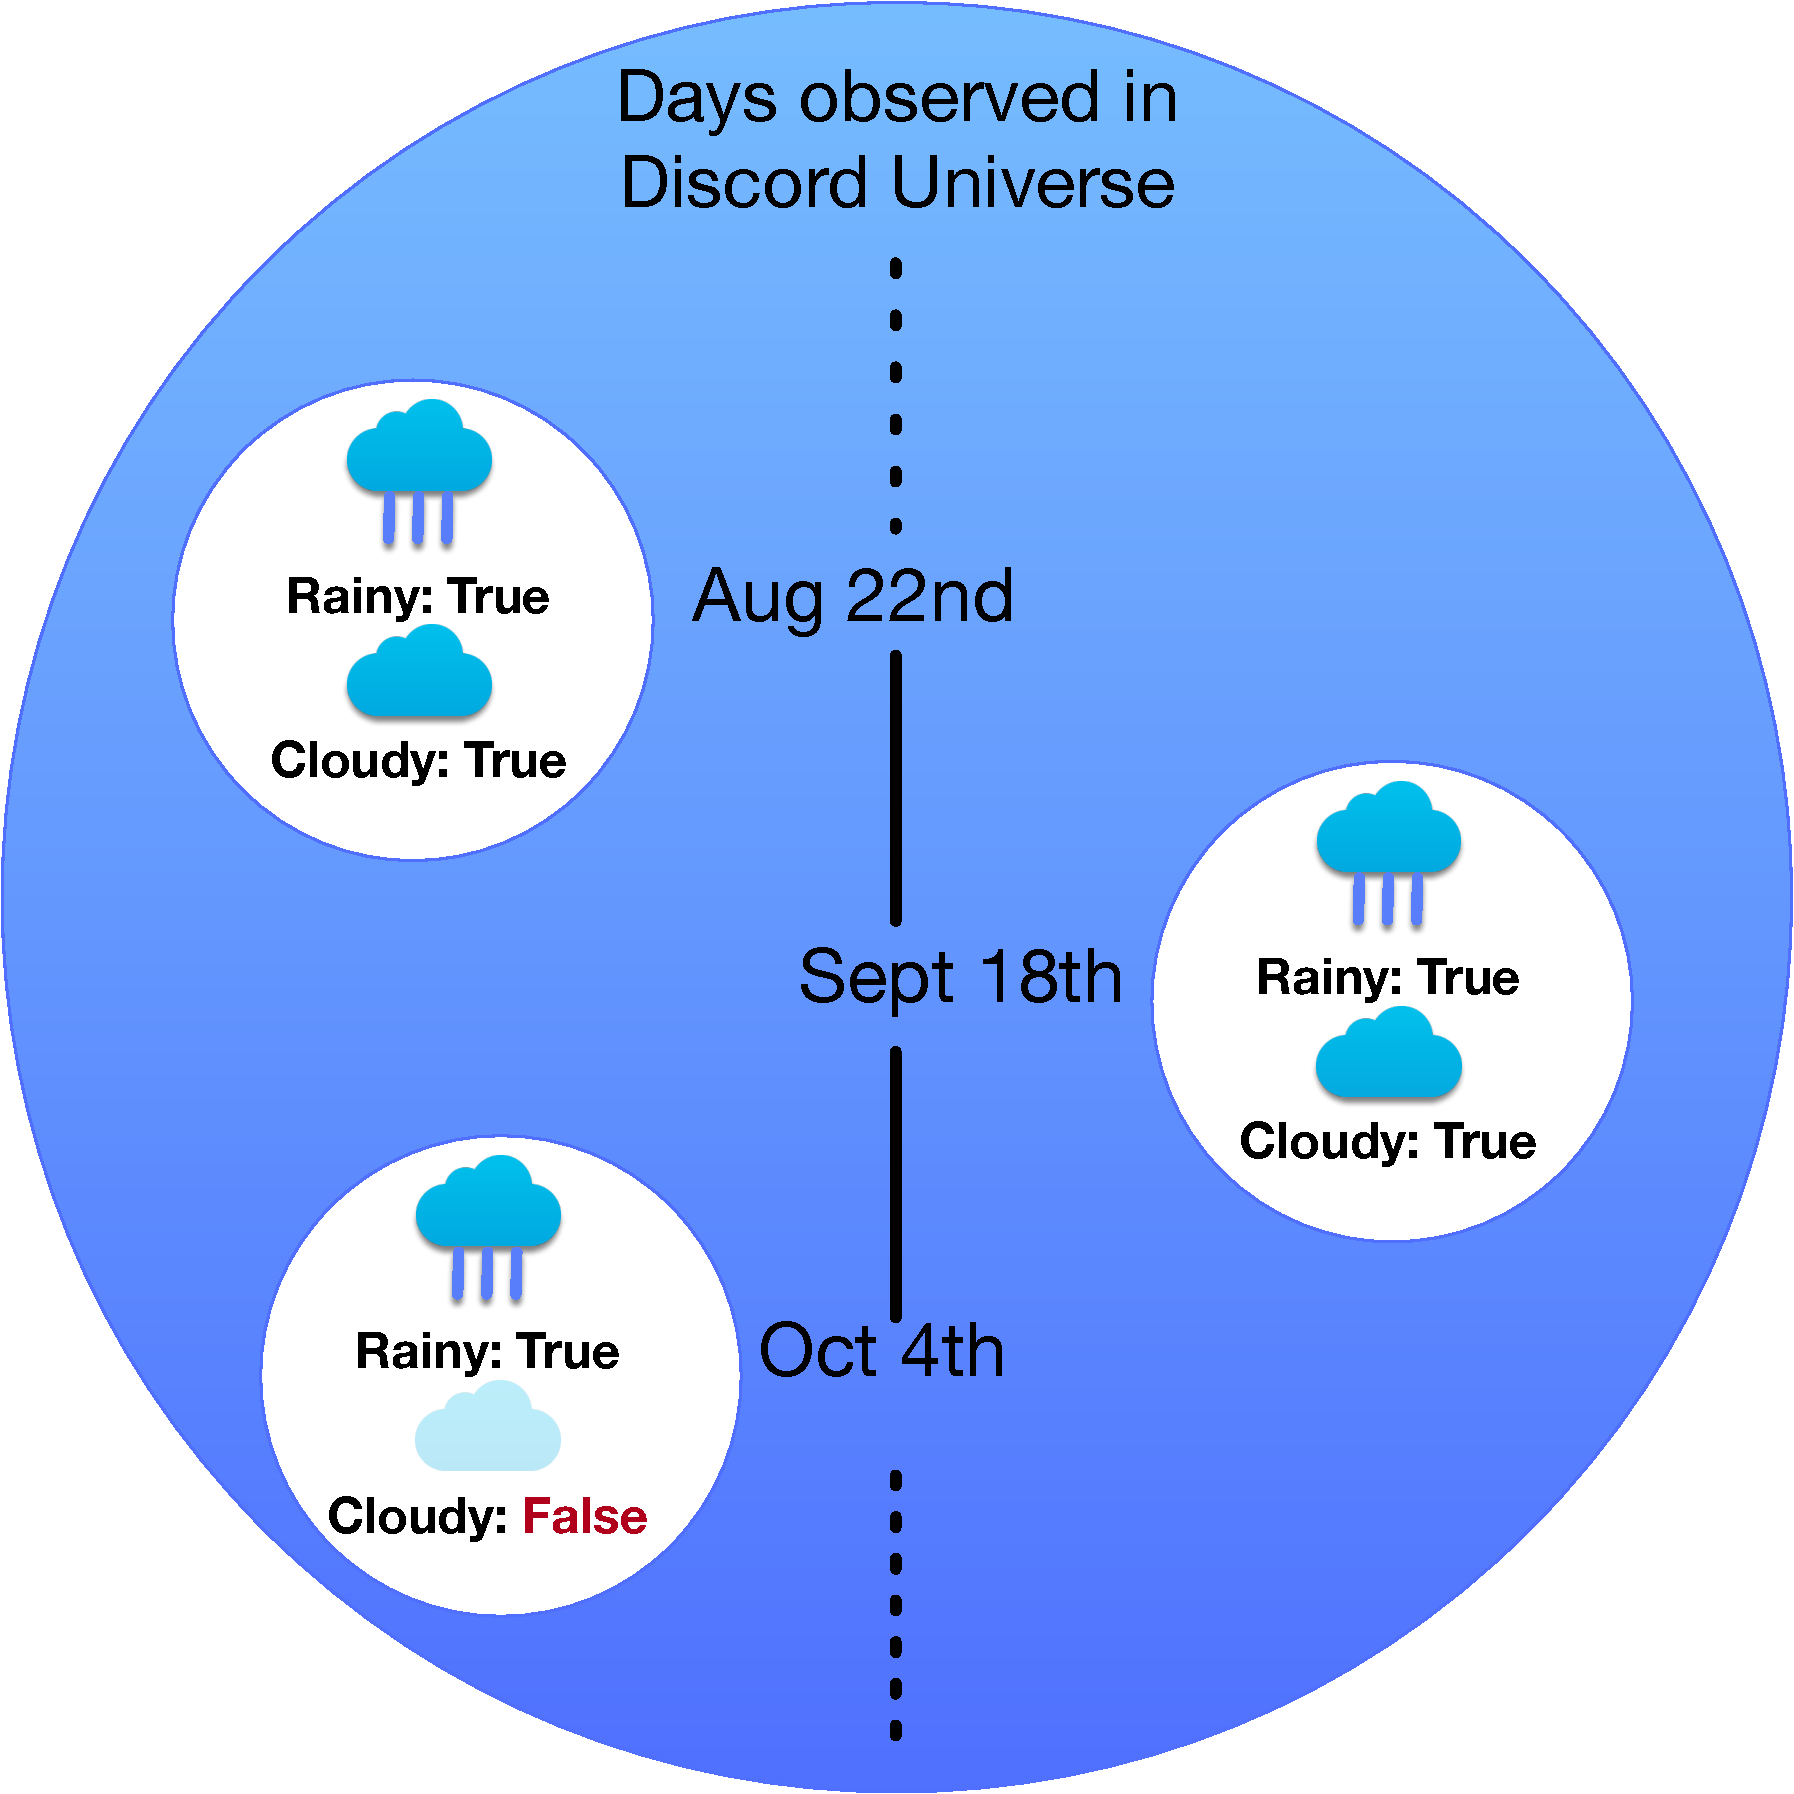
\includegraphics[width=1\textwidth]{./lectRDBMS/univQuantEx.pdf}\par}
\end{column}
\begin{column}{0.5\textwidth}

\begin{tabular}{|l|l|l|l|}  \hline
	& &  & \textrm{Raining(X)} \\ 
\textrm{Day} & \textrm{Rainy}& \textrm{Cloudy} & $\rightarrow$ \textrm{Cloudy(X)}\\ \hline
 &  & &  \\ \hline
 &  & &  \\ \hline
 &  & &  \\ \hline \hline
$\forall$  & &  & \\ \hline
\end{tabular}\\


\end{column}
\end{columns}

% Given this U of D, our statement is false

\end{frame}



%***********************************************************
\begin{frame}{Universal Quantification Example 2}

\begin{columns}
\begin{column}{0.5\textwidth}
\begin{itemize}
\item $\forall(X)(Friends(X,Y))$
\item This is a predicate over $Y$
\item Asserts that person Y is friends with everyone
\item Can be T or F, depending on what's in the U of D
\end{itemize}
\end{column}
\begin{column}{0.5\textwidth}

{\centering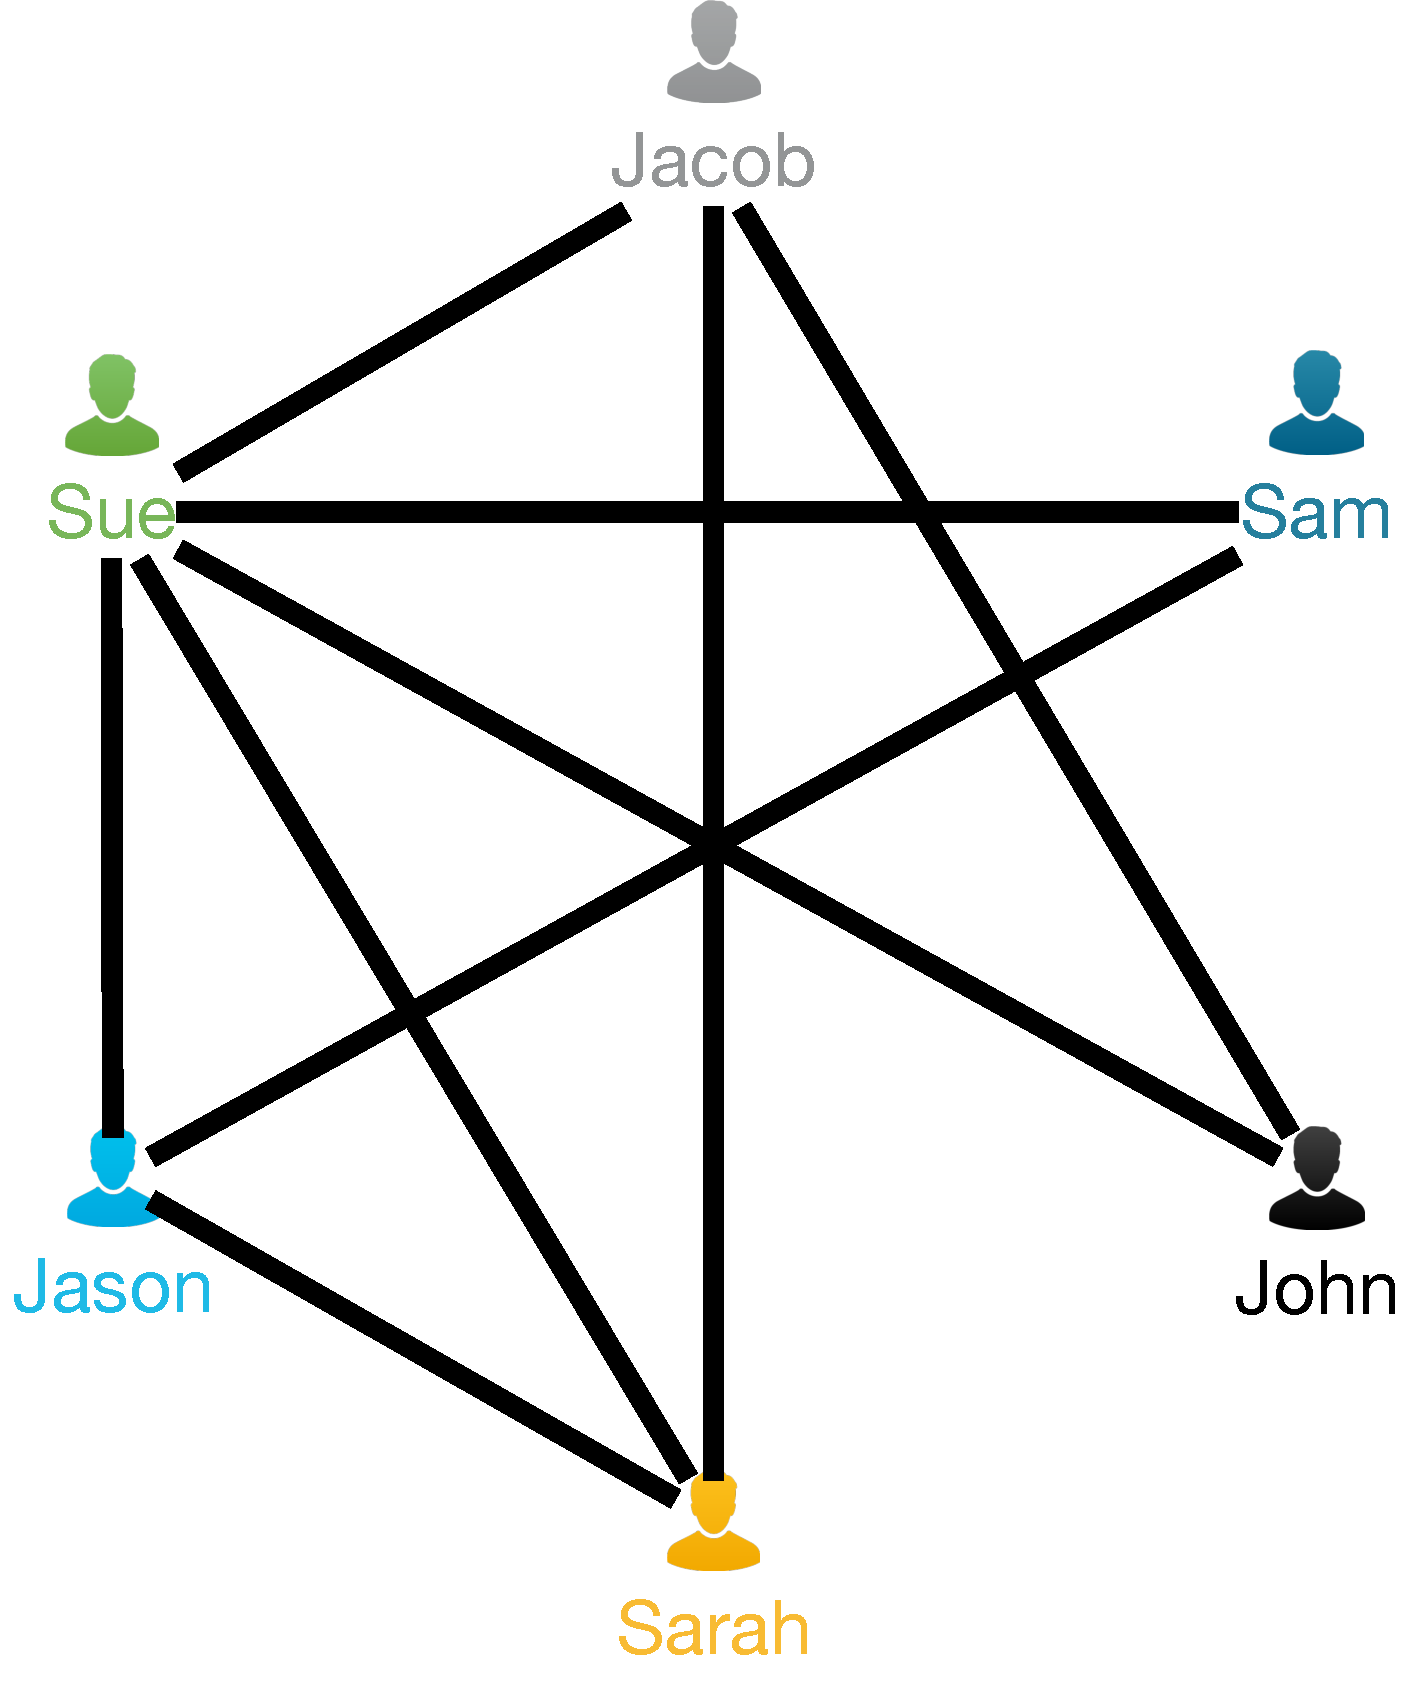
\includegraphics[width=.8\textwidth]{./lectRDBMS/friendNetwork.pdf}\par}
\end{column}
\end{columns}
\end{frame}

% True for Sue, F for everyone else
%complete set of objects available
%***********************************************************
\begin{frame}{Existential Quantification}

\begin{itemize}
\item Asserts that a predicate \textbf{can} be satisfied
\item Example:
	\begin{itemize}
	\item $\exists(X)(Raining(X) \wedge \neg Cloudy(X))$
	\item Asserts that it is possible for it to rain when it is not cloudy
	\item aka a ``sun shower"
	\end{itemize}
\end{itemize}
\end{frame}


%***********************************************************
\begin{frame}{Important Equivalence}

\begin{itemize}
\item $\forall(X)(P(X))$ is equivalent to...
\item $\neg \exists(X)(\neg P(X))$
	\begin{itemize}
	\item Ex: $\neg \exists(X,Y)(Friends(X,Y) \wedge Friends(X,Z) \wedge Friends(Y, Z))$
	\item Can be changed to:
	\item $\forall(X,Y)(\neg(Friends(X,Y) \wedge Friends(X,Z) \wedge Friends(Y, Z)))$
	\item Or $\forall(X,Y)( \neg Friends(X,Y) \vee \neg Friends(X,Z) \vee \neg Friends(Y, Z))$
	\end{itemize}
\item Which is easier?
	\begin{itemize}
	\item Often easier to reason about $\exists$ compared to $\forall$
	\item Can be hard to conceptualize an assertion that something is true over every
	item in the entire universe!
	\item In fact, SQL does not even have $\forall$
	\end{itemize}
\item[?] What is the name of rule applied to distribute the negation? % DeMorgan's Law
\end{itemize}
\end{frame}
	
%***********************************************************

\begin{frame}{Wrap up}
\begin{enumerate}
\item What is the fundamental benefit of the relational model?
\item Why does it matter?
\end{enumerate}

\begin{itemize}
	\item[?] How can we use what we learned today?
	\vspace{2em}
	\item[?] What do we know now that we didn't know before?
\end{itemize}


\end{frame}

\end{document}
